\documentclass{article}
% Choose a conveniently small page size
% PACKAGES
\usepackage[margin = 1in]{geometry}
\usepackage{amsfonts}
\usepackage{amsmath}
\usepackage{amssymb}
\usepackage{multicol}
\usepackage{graphicx}
\usepackage{float}
\usepackage{xcolor}
\usepackage{amsthm}
\usepackage{dsfont}
\usepackage{hyperref}

% MACROS
% Set Theory
\def\N{\mathbb{N}}
\def\R{\mathbb{R}}
\def\C{\mathbb{C}}
\def\Z{\mathbb{Z}}
%\def\^{\hat}
\def\-{\vec}
\def\d{\partial}
\def\!{\boldsymbol}
\def\X{\times}
%\def\-{\bar}
\def\bf{\textbf}
\def\l{\left}
\def\r{\right}
\title{Weekly Report}
\author{Damien}
\begin{document}
\maketitle
% \newpage
\section{Summary}
For this update I was tasked with looking at my implementation of the stopping conditions (18) and (19) of Chen et al. \cite{CHEN2013452} to determine whether they are appropriate or not. I was also asked to read Hu et al. \cite{hu2021adaptive} and \cite{su2019implicit} so that I can apply the code I currently have to the Boltzmann equation.
\section{Progress}
\subsection{Analyzing the Stopping Conditions}
The stopping conditions for Example 5.1.1 in Chen et al. \cite{CHEN2013452} are satisfied when
\begin{equation}\label{eq:cond1}
    \frac{\|u^{n+1} - u^n\| + h^p}{\|u^n - u^{n-1}\|} > 1
\end{equation}
and
\begin{equation}\label{eq:cond2}
    \|u^{n+1} - u^n\| - h^{p+1} < 0
\end{equation}
hold true. Here $p$ is the truncation error of the method. I set $p=3$ as it says in the paper. Call the condition in Equation \ref{eq:cond1} $c_1$ and the condition in Equation \ref{eq:cond2} $c_2$. In my code I have a while loop that runs while $\neg(c_1 \land c_2)$ which is logically equivalent to $\neg c_1 \lor \neg c_2$. This is the condition I originally had in my code. I just forgot the reasoning behind it during the meeting.
\begin{figure*}[h]
    \centering
    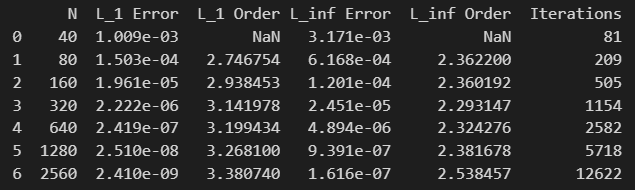
\includegraphics[width=0.5\textwidth]{imgs/5_1_1_table.png}
    \caption{This plot is an attempt to reproduce the results from Table 1 in Chen et al. This is the condition that I used in my code.}
\end{figure*}

I went on to plot the evolution of the $L_1$ error of the method. I got the following results.
\begin{figure}[H]
    \centering
    \begin{minipage}{.4\linewidth}
        \centering
        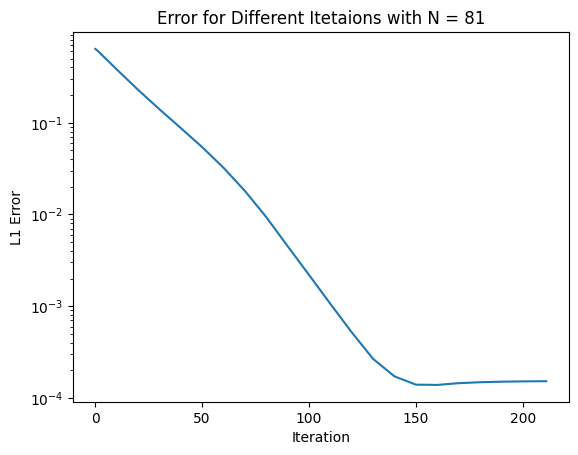
\includegraphics[width=\linewidth]{imgs/L1_81.png}
        % \subcaption{First subfigure}
    \end{minipage}
    \begin{minipage}{.4\linewidth}
        \centering
        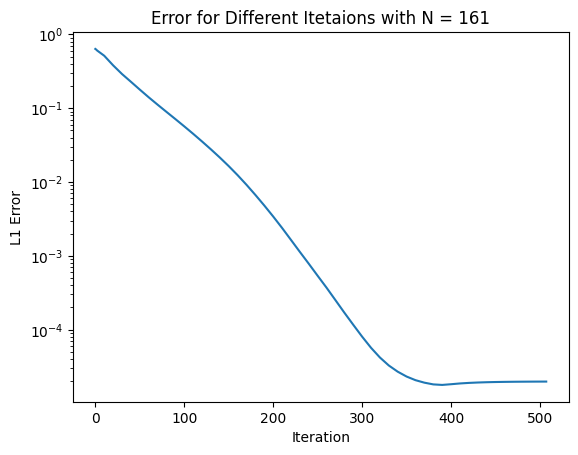
\includegraphics[width=\linewidth]{imgs/L1_161.png}
        % \subcaption{Second subfigure}
    \end{minipage}

    \begin{minipage}{.4\linewidth}
        \centering
        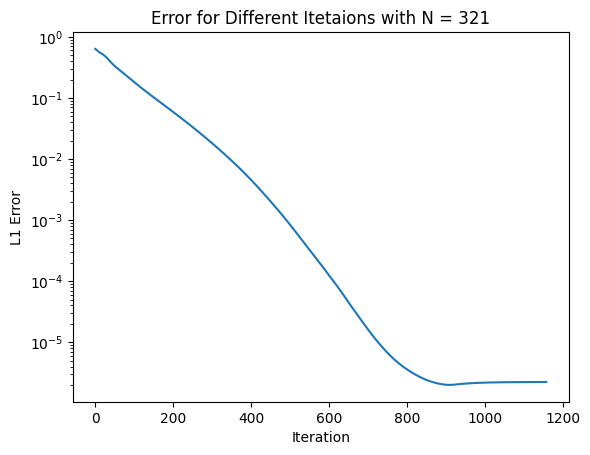
\includegraphics[width=\linewidth]{imgs/L1_321.png}
        % \subcaption{Third subfigure}
    \end{minipage}%
    \begin{minipage}{.4\linewidth}
        \centering
        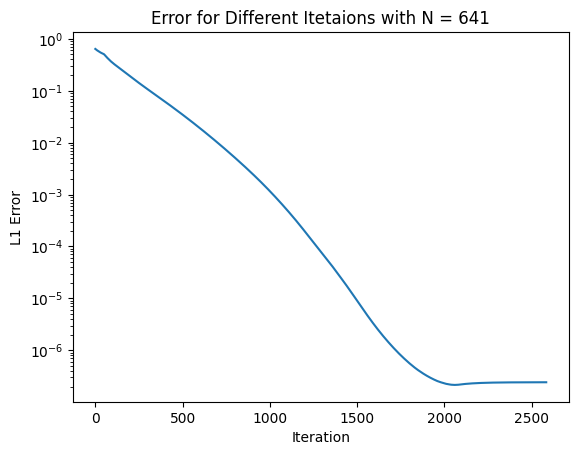
\includegraphics[width=\linewidth]{imgs/L1_641.png}
        % \subcaption{Fourth subfigure}
    \end{minipage}
    \caption{The shape of the error curve for the case of $N=80$ is similar to the right plot in Figure 2 of \cite{CHEN2013452}. The major differences are that the error here converges faster and my error curve has a long flat tail. This flat tail indicates that the method converged a good while before the stopping conditions were met. For this case at least the stopping conditions seem a bit conservative.}
    \label{fig:L1}
\end{figure}
\subsection{Reading}
There is a great deal of material in these two papers. It would help me to talk about precisely which sections I need to understand in order to achieve the next milestone. That being said, I came up with a list of questions about different parts of the reading.
\begin{enumerate}
    \item What sections of these papers should I thoroughly understand before continuing?
    \item What collision kernels should I test the method on? What should the boundary conditions, initial conditions, and solution domain be for the tests on these sample problems?
    \item Do I use the low-rank representation from Section 2 of Hu et al. \cite{hu2021adaptive} in my current implementation? If so, what basis should I use?
    \item I suppose the rank changing feature of Section 3 in Hu et al. \cite{hu2021adaptive} is irrelevant since we are only going for the steady state. Is this correct?
    \item I would like to see some references on the loss and gain term splitting in the collision operator in Su et al. \cite{su2019implicit}.
\end{enumerate}
% \subsubsection{Thoughts and Questions on Hu et al. \cite{hu2021adaptive}}
% \begin{enumerate}
    
% \end{enumerate}

\section{To Do}
I would like to meet and determine specific test problems so that I can get started on the implementation.
\bibliographystyle{plain}
\bibliography{refs}
\end{document}

% The orders and errors are almost exactly the same as the table produced with $p=3$. The only significant difference is that it took more sweeps to converge. I then began plotting the absolute value of the difference between the true solution and the approximation to see how the method was converging. This led to a surprising discovery. 
% \begin{figure}[H]
%     \centering
%     \begin{minipage}{.4\linewidth}
%         \centering
%         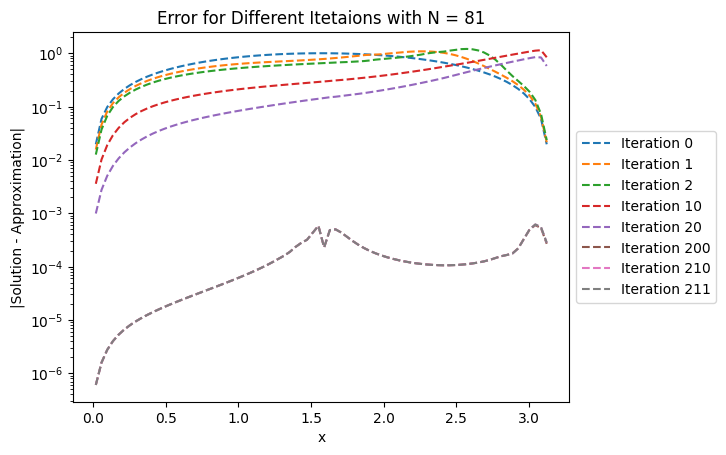
\includegraphics[width=\linewidth]{imgs/difference_81.png}
%         % \subcaption{First subfigure}
%     \end{minipage}%
%     \begin{minipage}{.4\linewidth}
%         \centering
%         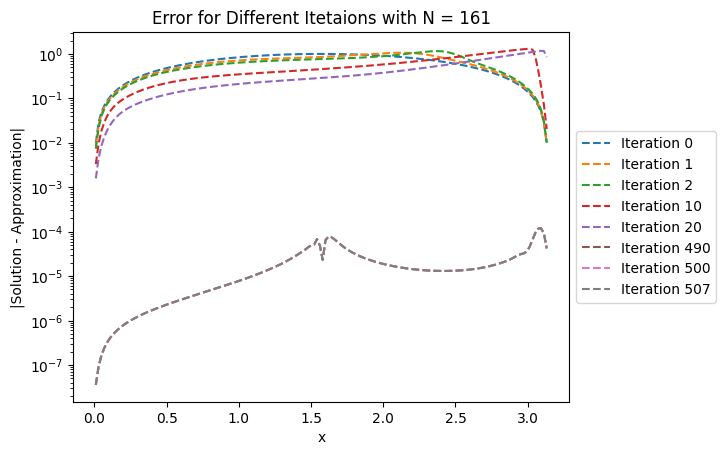
\includegraphics[width=\linewidth]{imgs/difference_161.png}
%         % \subcaption{Second subfigure}
%     \end{minipage}
%     \begin{minipage}{.4\linewidth}
%         \centering
%         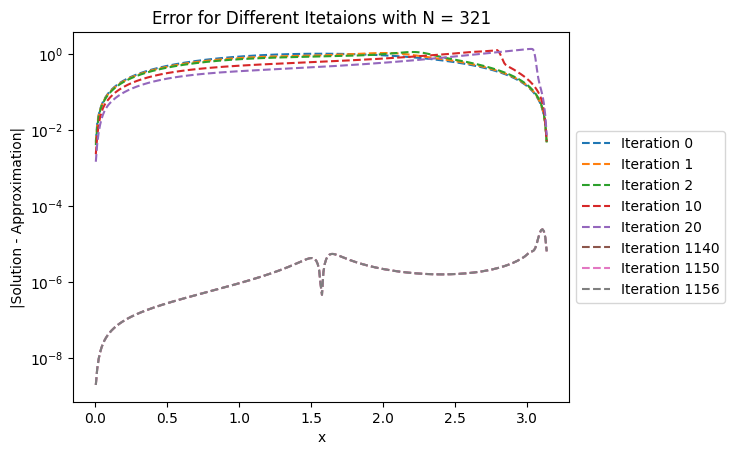
\includegraphics[width=\linewidth]{imgs/difference_321.png}
%         % \subcaption{Third subfigure}
%     \end{minipage}%
%     \begin{minipage}{.4\linewidth}
%         \centering
%         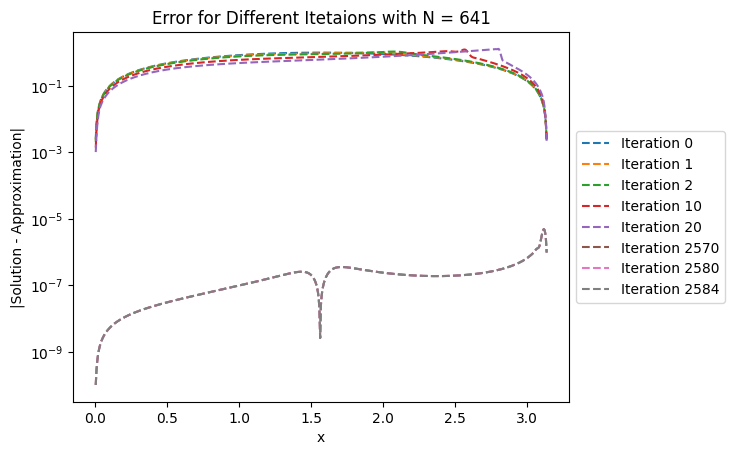
\includegraphics[width=\linewidth]{imgs/difference_641.png}
%         % \subcaption{Fourth subfigure}
%     \end{minipage}
%     \caption{Here we look at how the distribution of the error changes between iterations. We see that after two iterations the distribution remains relatively the same except for changes that are imperceptible even on a semi-log plot.}
%     \label{fig:difference}
% \end{figure}
% This is very strange and is entirely independent of the stopping criteria that we discussed above. In Equations \ref{eq:cond1} and \ref{eq:cond2} I took each $u^n$ to be the solution approximation after sweeping back and forth through the entire domain $n$ times. However, these error plots lead me to believe that this is not the case. Instead, I believe $u^n$ is the approximation after $n$ adjustments to the initial approximation. That is, if we have an approximation with $100$ interior points then sweeping once from left to right would give $u^{100}$. Then continuing on and sweeping from right to left would give $u^{200}$. In the way I was implementing the method previously I would have called this $u^1$ as opposed to $u^{200}$. Let us see how the plots look with this new labeling system.
% \begin{figure}[H]
%     \centering
%     \begin{minipage}{.4\linewidth}
%         \centering
%         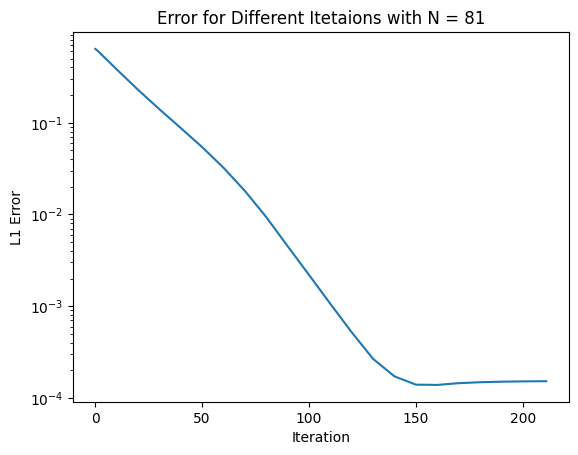
\includegraphics[width=\linewidth]{imgs/L1_81.png}
%     \end{minipage}%
%     \begin{minipage}{.4\linewidth}
%         \centering
%         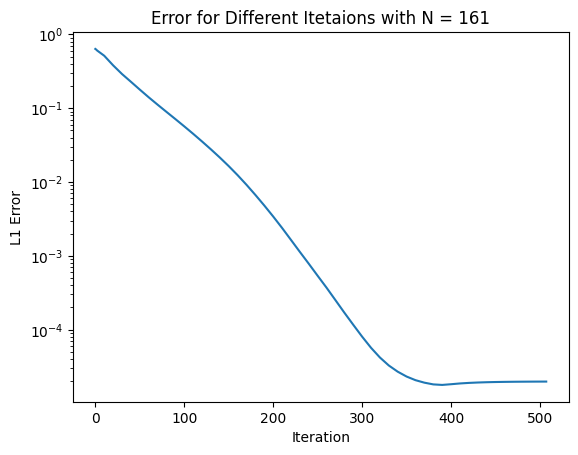
\includegraphics[width=\linewidth]{imgs/L1_161.png}
%     \end{minipage}

%     \begin{minipage}{.4\linewidth}
%         \centering
%         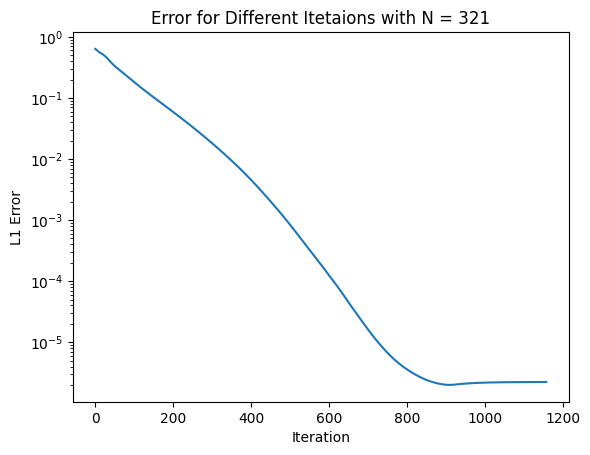
\includegraphics[width=\linewidth]{imgs/L1_321.png}
%     \end{minipage}%
%     \begin{minipage}{.4\linewidth}
%         \centering
%         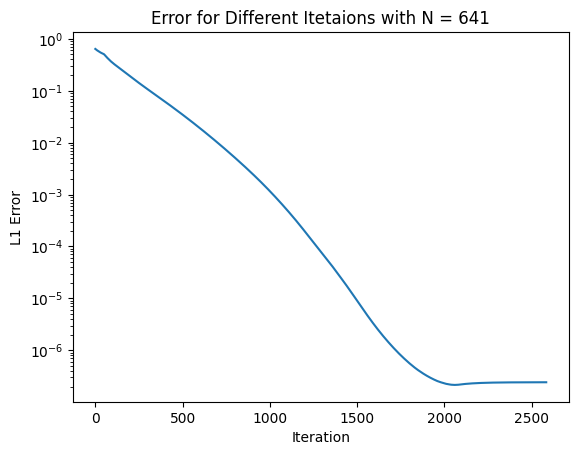
\includegraphics[width=\linewidth]{imgs/L1_641.png}
%     \end{minipage}
%     \caption{Each time the method is run it takes only two iterations to converge which is entirely different from the plots from Figure 2 in Chen et al. This is incredibly odd, especially since the error behaves the same for each resolution of collocation points. I also plotted the shape of the error function to get more detail on how the approximation matches the true solution.}
%     \label{fig:L1_adjusted}
% \end{figure}